\section{Application protocols}

Goal: E2E communication between servers and sensors using standard protocols,
possibly atop TCP/UDP/IP.

\subsection{Web services for IoT}

\begin{itemize}
		\item Web service technology allows integration with existing systems,
				libraries and knowledge
		\item Direct use of standard technologies (eg HTTP), or with
				translating proxies (eg COAP)
		\item Layer 7 protocols such as HTTP, COAP
		\item Atop of TCP/UDP
		\item Using XML, JSON, ... data formats
		\item With SOAP / REST APIs
\end{itemize}

\subsection{REST for IoT}

\begin{itemize}
		\item Resources encoded as representations
		\item Stateless, all state must be contained in request
		\item Use main HTTP verbs as operations
		\item XML or JSON as data format
\end{itemize}

HTTP verbs:
\begin{description}
		\item[GET] Retrieve resources
		\item[PUT] Update existing resource
		\item[POST] Create resource
		\item[DELETE] Delete resource
		\item[OPTIONS] Get allowed operations on resource
\end{description}

\subsection{COAP}

\begin{itemize}
		\item Subset of HTTP for constrained devices
		\item Short headers
		\item Built-in resource discovery and async messages
		\item Atop of datagram-oriented transport protocols such as UDP
		\item But with built-in reliable transmission
		\item Support for proxies and caching
		\item Can be statelessly mapped to and from HTTP
		\item Datagram-TLS for security
\end{itemize}

\subsubsection{Message types}

\begin{description}
		\item[Confirmable] Require response, piggybacked to ACK or async
				afterwards
		\item[Non-confirmable] Need neither be ACKed nor replied
		\item[Acknowledgement] Confirms reception of a message, may contain
				response to message
		\item[Reset] Sent if a confirmable message cannot be processed
\end{description}

\subsubsection{Request/Response interaction}

\begin{itemize}
		\item Request contains method, resource identifier, payload and media type
		\item Response contains result
		\item Request-response matching by token shared in both
\end{itemize}

\subsection{Frame format}

Version = 1, Type = 0 (conf), 1 (non-conf), 2 (ack), 3 (rst). TKL = token
length, 4 bit unsigned int length of token field (0 - 8 bytes).

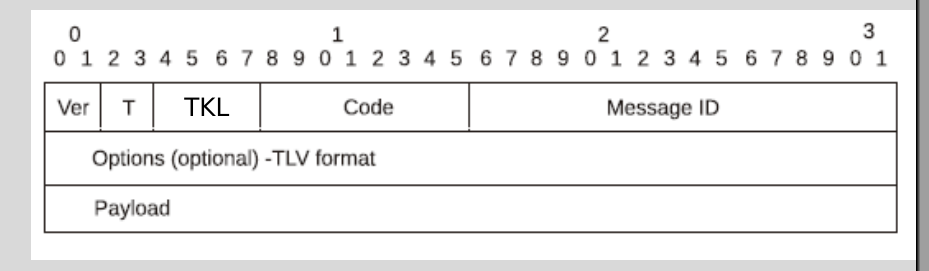
\includegraphics[width=0.5\textwidth]{10_coap}

\subsubsection{Observe functionality}

\begin{itemize}
		\item COAP has async `observation' approach to push information from
				server to client, unlike HTTP which is purely client-initiated
		\item Client can indicate its interest in update with a GET request
				with observe option set
		\item If server accepts, it will then push updates to the client (with
				sequence numbers for ordering) whenever the resource changes
		\item Updates contain client-specified token
\end{itemize}

\subsubsection{URIs}

\begin{itemize}
		\item Similar to HTTP URIs: `coap://host:port/path?query', host as IP or name.
\end{itemize}

\subsubsection{Service discovery}

\begin{itemize}
		\item Resource discovery using `.well-known' URIs
\end{itemize}

\subsection{MQTT, message queueing telemetry transport protocol}

\begin{itemize}
		\item Pub/Sub pattern
		\item Clients publish message to broker with a certain topic
		\item Clients can subscribe to topics, to receive messages published there
		\item Broker can optionally persist messages for e.g. future replay
		\item TCP as transport, TLS for security. MQTT has short 2-byte header and small payloads.
		\item Not for device-to-device transfer (payload limit) nor multicast traffic!
		\item Long-lived TCP connections required to keep overhead low»
\end{itemize}

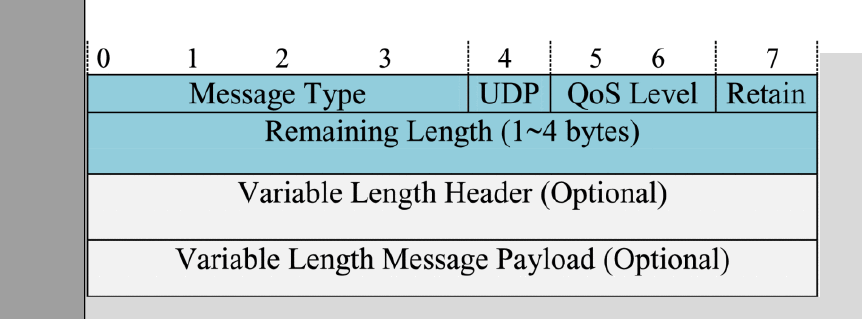
\includegraphics[width=0.5\textwidth]{10_mqtt}

\subsection{AMQP, advanced message queueing protocol}

\begin{itemize}
		\item Open protocol for message-oriented applications
		\item Reliable communication with guaranteed delivery, supporting
				at-most-once, at-least-once, exactly-once delivery
		\item Support for request/response as well as pub/sub
		\item Short fixed 8-byte header
		\item TCP as transport, TLS for security
		\item Clients create and post messages to exchanges
		\item Exchanges route messages to queues bsaed on defined rules
		\item Receivers create queues and receive messages from there
\end{itemize}

\subsection{Data distribution service, DDS}

\begin{itemize}
		\item Pub/sub protocol for real-time M2M communication
		\item Broker-less architecture, decentralized, P2P communication
		\item QoS policies
		\item Discovery allowing subscribers to find publishers in GDS (global data space)
\end{itemize}
